\documentclass[tikz,border=2pt]{standalone}
\usepackage{tikz}
\usetikzlibrary{positioning}
\begin{document}
	\begin{tikzpicture}[
	main/.style={rectangle, rounded corners, text centered, text width=3cm, draw=black},
	aux/.style={}
	]	
	
	\node (project) [main] {Project};
	

		
		\node (sim) [main, below=of project] {Simulation};
	
		\node (multiagent) [main, left= of sim] {Multi-agent case};
	
		\node (control) [main, left= of multiagent] {Quad Control};

		\node (mod) [main, left= of control] {Modelling};
					
		\node (lit) [main, left=of mod] {Literature};
		
		\node (results) [main, right= of sim] {Results and conclusions};	
		\node (rep) [main, right=of results] {Report};
		\node (peerrev) [main, right=of rep] {Peer-Review};
		\node (presentation) [main, right=of peerrev] {Presentation};	

	\draw [-latex] (project.south)--++(0,-.3)-| (lit.north);
	\draw [-latex] (project.south)--++(0,-.3)-| (mod.north);
	\draw [-latex] (project.south)--++(0,-.3)-| (sim.north);
	\draw [-latex] (project.south)--++(0,-.3)-| (results.north);
	\draw [-latex] (project.south)--++(0,-.3)-| (rep.north);
	\draw [-latex] (project.south)--++(0,-.3)-| (peerrev.north);
	\draw [-latex] (project.south)--++(0,-.3)-| (control.north);
	\draw [-latex] (project.south)--++(0,-.3)-| (multiagent.north);
	\draw [-latex] (project.south)--++(0,-.3)-| (presentation.north);
	
	
	\end{tikzpicture}
\end{document}